\documentclass[a4paper, 11pt]{article}
\usepackage{graphicx}
\usepackage{multicol}
\usepackage{tabularx}
\usepackage{enumitem}
\usepackage[a4paper, margin=1.8cm]{geometry}
\usepackage{listings}
\usepackage{amssymb}
\usepackage{gvv}
\usepackage{gvv-book}
\usepackage{amsmath}
\usepackage{setspace}
\usepackage{caption}
\usepackage{tfrupee}
\usepackage{float}

\graphicspath{./figs}

\begin{document}

\begin{center}
    \huge{GATE 2023}\\
    \large{Electronics and Communication Engineering \brak{EC}}\\
    \large{EE25BTECH11041 - Naman Kumar}
\end{center}

\section*{General Aptitude \brak{GA}}

\begin{enumerate}
    \item I cannot support this proposal. My \underline{\hspace{2cm}} will not permit it.
    \begin{enumerate}
    \begin{multicols}{4}
        \item conscious
        \item consensus
        \item conscience
        \item consent
    \end{multicols}
    \end{enumerate}
    
    \hfill{\brak{\text{GATE EC 2023}}}
    
    \item Parliament $\colon$ Legislature :: Courts $\colon \underline{\hspace{2cm}} \brak{\text{By word meaning}}$
    \begin{enumerate}
    \begin{multicols}{4}
        \item Judiciary
        \item Executive
        \item Governmental
        \item Legal
    \end{multicols}
    \end{enumerate}
    
    \hfill{\brak{\text{GATE EC 2023}}}
    
    \item What is the smallest number with distinct digits whose digits add up to $45$?
    \begin{enumerate}
    \begin{multicols}{2}
        \item $123555789$
        \item $123457869$
        \item $123456789$
        \item $99999$
    \end{multicols}
    \end{enumerate}
    
    \hfill{\brak{\text{GATE EC 2023}}}
    
    \item In a class of $100$ students,
    \begin{enumerate}[label=\brak{\roman*}]
        \item there are $30$ students who neither like romantic movies nor comedy movies,
        \item the number of students who like romantic movies is twice the number of students who like comedy movies, and
        \item the number of students who like both romantic movies and comedy movies is $20$.
    \end{enumerate}
    How many students in the class like romantic movies?
    
    \begin{enumerate}
    \begin{multicols}{2}
        \item $40$
        \item $20$
        \item $60$
        \item $30$
    \end{multicols}
    \end{enumerate}
    
    \hfill{\brak{\text{GATE EC 2023}}}
    
    \item How many rectangles are present in the given figure?
    \begin{figure}[H]
        \centering
        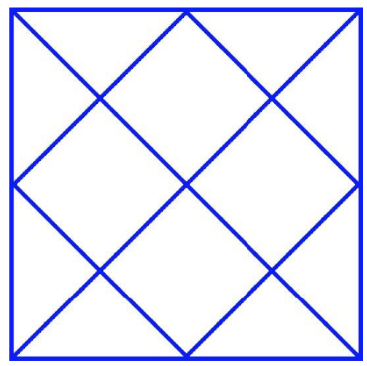
\includegraphics[width=0.3\columnwidth]{figs/GA5.png}
        \caption*{}
        \label{fig:q5}
    \end{figure}
    
    \begin{enumerate}
    \begin{multicols}{4}
        \item $8$
        \item $9$
        \item $10$
        \item $12$
    \end{multicols}
    \end{enumerate}
    
    \hfill{\brak{\text{GATE EC 2023}}}
    
    \item Forestland is a planet inhabited by different kinds of creatures. Among other creatures, it is populated by animals all of whom are ferocious. There are also creatures that have claws, and some that do not. All creatures that have claws are ferocious.
    Based only on the information provided above, which one of the following options can be logically inferred with certainty?
    
    \begin{enumerate}
        \item All creatures with claws are animals.
        \item Some creatures with claws are non-ferocious.
        \item Some non-ferocious creatures have claws.
        \item Some ferocious creatures are creatures with claws.
    \end{enumerate}
    
    \hfill{\brak{\text{GATE EC 2023}}}
    
    \item Which one of the following options represents the given graph?
    \begin{figure}[H]
        \centering
        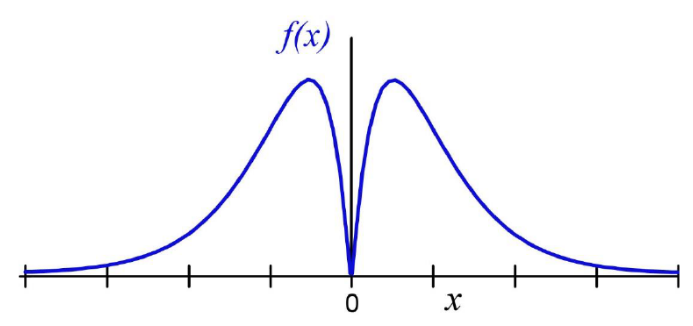
\includegraphics[width=0.4\columnwidth]{figs/GA7.png}
        \caption*{}
        \label{fig:q7}
    \end{figure}
    
    \begin{enumerate}
    \begin{multicols}{2}
        \item $f(x)=x^{2}2^{-\abs{x}}$
        \item $f(x)=x 2^{-\abs{x}}$
        \item $f(x)=\abs{x}2^{-x}$
        \item $f(x)=x 2^{-x}$
    \end{multicols}
    \end{enumerate}
    
    \hfill{\brak{\text{GATE EC 2023}}}

    \item Which one of the following options can be inferred from the given passage alone?
    \begin{quote}
    When I was a kid, I was partial to stories about other worlds and interplanetary travel. I used to imagine that I could just gaze off into space and be whisked to another planet.
    \end{quote}
    \brak{\text{Excerpt from The Truth about Stories by T. King}}

    \begin{enumerate}
        \item It is a child's description of what he or she likes.
        \item It is an adult's memory of what he or she liked as a child.
        \item The child in the passage read stories about interplanetary travel only in parts.
        \item It teaches us that stories are good for children.
    \end{enumerate}
    
    \hfill{\brak{\text{GATE EC 2023}}}
    
    \item Out of $1000$ individuals in a town, $100$ unidentified individuals are covid positive. Due to lack of adequate covid-testing kits, the health authorities of the town devised a strategy to identify these covid-positive individuals. The strategy is to:
    \begin{enumerate}[label=\brak{\roman*}]
        \item Collect saliva samples from all $1000$ individuals and randomly group them into sets of $5$.
        \item Mix the samples within each set and test the mixed sample for covid.
        \item If the test done in \brak{ii} gives a negative result, then declare all the $5$ individuals to be covid negative.
        \item If the test done in \brak{ii} gives a positive result, then all the $5$ individuals are separately tested for covid.
    \end{enumerate}
    Given this strategy, no more than \underline{\hspace{2cm}} testing kits will be required to identify all the $100$ covid positive individuals irrespective of how they are grouped.
    
    \begin{enumerate}
    \begin{multicols}{2}
        \item $700$
        \item $600$
        \item $800$
        \item $1000$
    \end{multicols}
    \end{enumerate}

    \hfill{\brak{\text{GATE EC 2023}}}
    
    \item A $100\text{ cm} \times 32\text{ cm}$ rectangular sheet is folded $5$ times. Each time the sheet is folded, the long edge aligns with its opposite side. Eventually, the folded sheet is a rectangle of dimensions $100\text{ cm} \times 1\text{ cm}$.
    
    The total number of creases visible when the sheet is unfolded is \underline{\hspace{2cm}}.
    
    \begin{enumerate}
    \begin{multicols}{2}
        \item $32$
        \item $5$
        \item $31$
        \item $63$
    \end{multicols}
    \end{enumerate}

    \hfill{\brak{\text{GATE EC 2023}}}

\end{enumerate}

\section*{Electronics and Communication Engineering \brak{EC}}
\begin{enumerate}
    \item Let $v_1 = \myvec{1 \\ 2 \\ 0}$ and $v_2 = \myvec{2 \\ 1 \\ 3}$ be two vectors. The value of the coefficient $\alpha$ in the expression $v_1 = \alpha v_2 + e$, which minimizes the length of the error vector $e$, is
    
    \begin{enumerate}
    \begin{multicols}{2}
        \item $\frac{7}{2}$
        \item $-\frac{2}{7}$
        \item $\frac{2}{7}$
        \item $-\frac{7}{2}$
    \end{multicols}
    \end{enumerate}
    
    \hfill{\brak{\text{GATE EC 2023}}}
    
    \item The rate of increase, of a scalar field $f(x,y,z) = xyz$, in the direction $v=\brak{2,1,2}$ at a point $\brak{0,2,1}$ is
    
    \begin{enumerate}
    \begin{multicols}{2}
        \item $\frac{2}{3}$
        \item $\frac{4}{3}$
        \item $2$
        \item $4$
    \end{multicols}
    \end{enumerate}
    
    \hfill{\brak{\text{GATE EC 2023}}}

    \item Let $w^4 = 16j$. Which of the following cannot be a value of $w$?
    
    \begin{enumerate}
    \begin{multicols}{2}
        \item $2e^{j\frac{2\pi}{8}}$
        \item $2e^{j\frac{\pi}{8}}$
        \item $2e^{j\frac{5\pi}{8}}$
        \item $2e^{j\frac{9\pi}{8}}$
    \end{multicols}
    \end{enumerate}
    
    \hfill{\brak{\text{GATE EC 2023}}}
    
    \item The value of the contour integral, $\oint_C \brak{\frac{z+2}{z^2+2z+2}}dz$ where the contour C is $\{z \colon \abs{z+1-\frac{3}{2}j}=1\}$, taken in the counter clockwise direction, is
    
    \begin{enumerate}
    \begin{multicols}{2}
        \item $-\pi\brak{1+j}$
        \item $\pi\brak{1+j}$
        \item $\pi\brak{1-j}$
        \item $-\pi\brak{1-j}$
    \end{multicols}
    \end{enumerate}
    
    \hfill{\brak{\text{GATE EC 2023}}}
    
    \item Let the sets of eigenvalues and eigenvectors of a matrix B be $\{\lambda_k | 1 \le k \le n\}$ and $\{v_k | 1 \le k \le n\}$, respectively. For any invertible matrix P, the sets of eigenvalues and eigenvectors of the matrix A, where $B = P^{-1}AP$, respectively, are
    
    \begin{enumerate}
    \begin{multicols}{2}
        \item $\{\lambda_k \det\brak{A} | 1 \le k \le n\}$ and $\{Pv_k | 1 \le k \le n\}$
        \item $\{\lambda_k | 1 \le k \le n\}$ and $\{v_k | 1 \le k \le n\}$
        \item $\{\lambda_k | 1 \le k \le n\}$ and $\{Pv_k | 1 \le k \le n\}$
        \item $\{\lambda_k | 1 \le k \le n\}$ and $\{P^{-1}v_k | 1 \le k \le n\}$
    \end{multicols}
    \end{enumerate}
    
    \hfill{\brak{\text{GATE EC 2023}}}
    
    \item In a semiconductor, if the Fermi energy level lies in the conduction band, then the semiconductor is known as
    
    \begin{enumerate}
    \begin{multicols}{2}
        \item degenerate n-type.
        \item degenerate p-type.
        \item non-degenerate n-type.
        \item non-degenerate p-type.
    \end{multicols}
    \end{enumerate}
    
    \hfill{\brak{\text{GATE EC 2023}}}
    
    \item For an intrinsic semiconductor at temperature $T=0$ K, which of the following statement is true?
    
    \begin{enumerate}
        \item All energy states in the valence band are filled with electrons and all energy states in the conduction band are empty of electrons.
        \item All energy states in the valence band are empty of electrons and all energy states in the conduction band are filled with electrons.
        \item All energy states in the valence and conduction band are filled with holes.
        \item All energy states in the valence and conduction band are filled with electrons.
    \end{enumerate}
    
    \hfill{\brak{\text{GATE EC 2023}}}
    
    \item A series RLC circuit has a quality factor Q of $1000$ at a center frequency of $10^6$ rad/s. The possible values of R, L and C are
    
    \begin{enumerate}
    \begin{multicols}{2}
        \item $R=1 \ohm$, $L=1 \mu H$ and $C=1 \mu F$
        \item $R=0.1 \ohm$, $L=1 \mu H$ and $C=1 \mu F$
        \item $R=0.01 \ohm$, $L=1 \mu H$ and $C=1 \mu F$
        \item $R=0.001 \ohm$, $L=1 \mu H$ and $C=1 \mu F$
    \end{multicols}
    \end{enumerate}
    
    \hfill{\brak{\text{GATE EC 2023}}}
    
    \item For a MOS capacitor, $V_{fb}$ and $V_t$ are the flat-band voltage and the threshold voltage, respectively. The variation of the depletion width $\brak{W_{dep}}$ for varying gate voltage $\brak{V_g}$ is best represented by
    
    \begin{enumerate}
        \item \begin{figure}[H] \centering 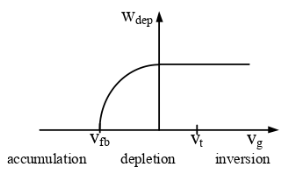
\includegraphics[width=0.45\columnwidth]{figs/Q9A.png} \caption*{} \label{fig:q19a} \end{figure}
        \item \begin{figure}[H] \centering 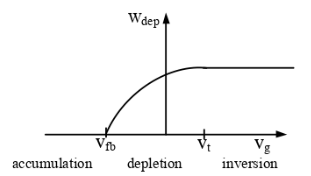
\includegraphics[width=0.45\columnwidth]{figs/Q9B.png} \caption*{} \label{fig:q19b} \end{figure}
        \item \begin{figure}[H] \centering 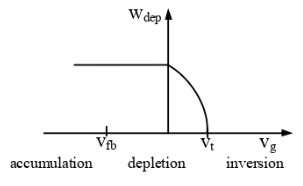
\includegraphics[width=0.45\columnwidth]{figs/Q9C.png} \caption*{} \label{fig:q19c} \end{figure}
        \item \begin{figure}[H] \centering 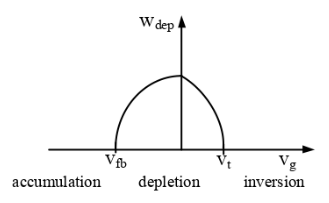
\includegraphics[width=0.45\columnwidth]{figs/Q9D.png} \caption*{} \label{fig:q19d} \end{figure}
    \end{enumerate}
    
    \hfill{\brak{\text{GATE EC 2023}}}
    
    \item Consider a narrow band signal, propagating in a lossless dielectric medium $\brak{\epsilon_r = 4, \mu_r = 1}$, with phase velocity $v_p$ and group velocity $v_g$. Which of the following statement is true? \brak{c is the velocity of light in vacuum.}
    
    \begin{enumerate}
    \begin{multicols}{2}
        \item $v_p > c$, $v_g > c$
        \item $v_p < c$, $v_g > c$
        \item $v_p > c$, $v_g < c$
        \item $v_p < c$, $v_g < c$
    \end{multicols}
    \end{enumerate}
    
    \hfill{\brak{\text{GATE EC 2023}}}

    \item In the circuit shown below, $V_I$ and $V_2$ are bias voltages. Based on input and output impedances, the circuit behaves as a
    \begin{figure}[H]
        \centering
        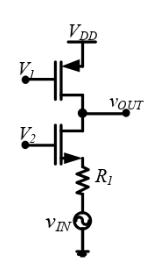
\includegraphics[width=0.4\columnwidth]{figs/Q11.png}
        \caption*{}
        \label{fig:q21}
    \end{figure}
    \begin{enumerate}
        \item voltage controlled voltage source.
        \item voltage controlled current source.
        \item current controlled voltage source.
        \item current controlled current source.
    \end{enumerate}
    
    \hfill{\brak{\text{GATE EC 2023}}}
    
    \item A cascade of common-source amplifiers in a unity gain feedback configuration oscillates when
    \begin{enumerate}
        \item the closed loop gain is less than $1$ and the phase shift is less than $180\degree$
        \item the closed loop gain is greater than $1$ and the phase shift is less than $180\degree$.
        \item the closed loop gain is less than $1$ and the phase shift is greater than $180\degree$.
        \item the closed loop gain is greater than $1$ and the phase shift is greater than $180\degree$.
    \end{enumerate}

    \hfill{\brak{\text{GATE EC 2023}}}
    
    \item In the circuit shown below, P and Q are the inputs. The logical function realized by the circuit shown below is
    \begin{figure}[H]
        \centering
        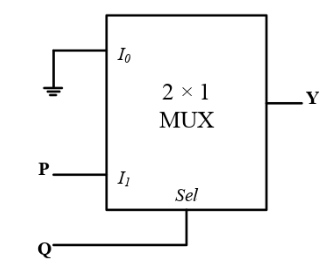
\includegraphics[width=0.3\columnwidth]{figs/Q13.png}
        \caption*{}
        \label{fig:q23}
    \end{figure}
    \begin{enumerate}
    \begin{multicols}{2}
        \item $Y = PQ$
        \item $Y = P+Q$
        \item $Y = \overline{PQ}$
        \item $Y = \overline{P+Q}$
    \end{multicols}
    \end{enumerate}

    \hfill{\brak{\text{GATE EC 2023}}}
    
    \item The synchronous sequential circuit shown below works at a clock frequency of $1$ GHz. The throughput, in Mbits/s, and the latency, in ns, respectively, are
    \begin{figure}[H]
        \centering
        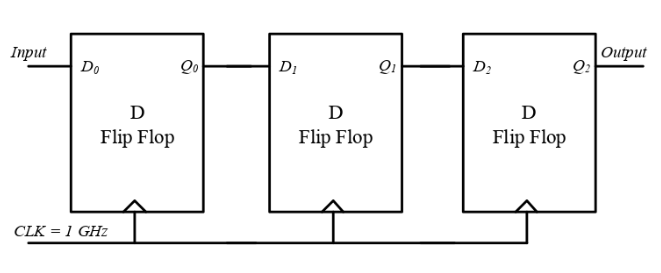
\includegraphics[width=0.7\columnwidth]{figs/Q14.png}
        \caption*{}
        \label{fig:q24}
    \end{figure}
    \begin{enumerate}
    \begin{multicols}{2}
        \item $1000, 3$
        \item $333.33, 1$
        \item $2000, 3$
        \item $333.33, 3$
    \end{multicols}
    \end{enumerate}
    
    \hfill{\brak{\text{GATE EC 2023}}}
    
    \item The open loop transfer function of a unity negative feedback system is
    \[G(s) = \frac{k}{s(1+sT_1)(1+sT_2)}\]
    where k, $T_1$ and $T_2$ are positive constants. The phase cross-over frequency, in rad/s, is
    \begin{enumerate}
    \begin{multicols}{2}
        \item $\frac{1}{\sqrt{T_1 T_2}}$
        \item $\frac{1}{T_1 T_2}$
        \item $\frac{1}{T_1 \sqrt{T_2}}$
        \item $\frac{1}{T_2 \sqrt{T_1}}$
    \end{multicols}
    \end{enumerate}

    \hfill{\brak{\text{GATE EC 2023}}}
    
    \item Consider a system with input $x(t)$ and output $y(t) = x(e^t)$. The system is
    \begin{enumerate}
    \begin{multicols}{2}
        \item Causal and time invariant.
        \item Non-causal and time varying.
        \item Causal and time varying.
        \item Non-causal and time invariant.
    \end{multicols}
    \end{enumerate}

    \hfill{\brak{\text{GATE EC 2023}}}
    
    \item Let $m(t)$ be a strictly band-limited signal with bandwidth B and energy E. Assuming $\omega_0 = 10B$, the energy in the signal $m(t) \cos \omega_0 t$ is
    \begin{enumerate}
    \begin{multicols}{2}
        \item $\frac{E}{4}$
        \item $\frac{E}{2}$
        \item E
        \item 2E
    \end{multicols}
    \end{enumerate}
    
    \hfill{\brak{\text{GATE EC 2023}}}

    \item The Fourier transform $X(\omega)$ of $x(t) = e^{-t^2}$ is
    
    Note: $\int_{-\infty}^{\infty} e^{-y^2} dy = \sqrt{\pi}$
    
    \begin{enumerate}
    \begin{multicols}{2}
        \item $\sqrt{\pi} e^{\frac{\omega^2}{2}}$
        \item $\frac{e^{-\frac{\omega^2}{4}}}{2\sqrt{\pi}}$
        \item $\sqrt{\pi} e^{-\frac{\omega^2}{4}}$
        \item $\sqrt{\pi} e^{-\frac{\omega^2}{2}}$
    \end{multicols}
    \end{enumerate}
    
    \hfill{\brak{\text{GATE EC 2023}}}

    \item In the table shown below, match the signal type with its spectral characteristics.
    
    \begin{table}[H]
        \centering
        \begin{tabular}{ll}
            \textbf{Signal type} & \textbf{Spectral characteristics} \\
            (i) Continuous, aperiodic & (a) Continuous, aperiodic \\
            (ii) Continuous, periodic & (b) Continuous, periodic \\
            (iii) Discrete, aperiodic & (c) Discrete, aperiodic \\
            (iv) Discrete, periodic & (d) Discrete, periodic \\
        \end{tabular}
        \caption*{}
    \end{table}

    \begin{enumerate}
        \item (i)$\rightarrow$(a), (ii)$\rightarrow$(b), (iii)$\rightarrow$(c), (iv)$\rightarrow$(d)
        \item (i)$\rightarrow$(a), (ii)$\rightarrow$(c), (iii)$\rightarrow$(b), (iv)$\rightarrow$(d)
        \item (i)$\rightarrow$(d), (ii)$\rightarrow$(b), (iii)$\rightarrow$(c), (iv)$\rightarrow$(a)
        \item (i)$\rightarrow$(a), (ii)$\rightarrow$(c), (iii)$\rightarrow$(d), (iv)$\rightarrow$(b)
    \end{enumerate}
    
    \hfill{\brak{\text{GATE EC 2023}}}

    \item For a real signal, which of the following is/are valid power spectral density/densities?

    \begin{enumerate}
        \item $S_x(\omega) = \frac{2}{9+\omega^2}$
        \item $S_x(\omega) = e^{-\omega^2}\cos^2\omega$
        \item \begin{figure}[H] \centering 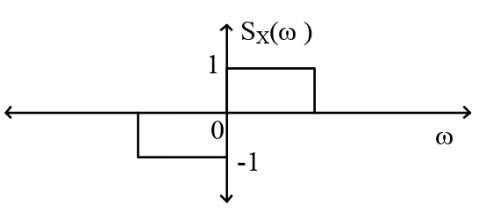
\includegraphics[width=0.3\columnwidth]{figs/Q20C.png} \caption*{} \label{fig:q30c} \end{figure}
        \item \begin{figure}[H] \centering 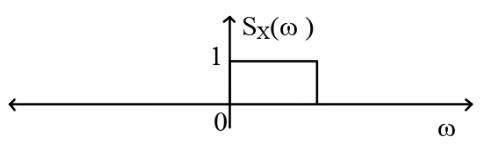
\includegraphics[width=0.3\columnwidth]{figs/Q20D.png} \caption*{} \label{fig:q30d} \end{figure}
    \end{enumerate}

    \hfill{\brak{\text{GATE EC 2023}}}
    
    \item The signal-to-noise ratio \brak{SNR} of an ADC with a full-scale sinusoidal input is given to be $61.96$ dB. The resolution of the ADC is \underline{\hspace{2cm}} bits \brak{\text{rounded off to the nearest integer}}.
    
    \hfill{\brak{\text{GATE EC 2023}}}
    
    \item In the circuit shown below, the current $i$ flowing through 200 $\Omega$ resistor is \underline{\hspace{2cm}} mA \brak{rounded off to two decimal places}.
    \begin{figure}[H]
        \centering
        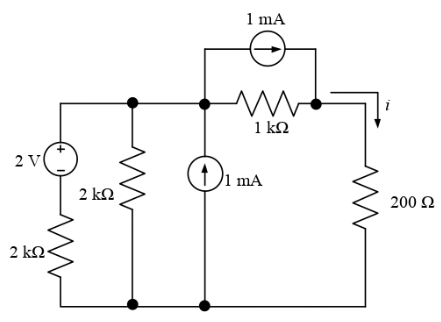
\includegraphics[width=0.5\columnwidth]{figs/Q22.png}
        \caption*{}
        \label{fig:q32}
    \end{figure}
    
    \hfill{\brak{\text{GATE EC 2023}}}
    
    \item For the two port network shown below, the [Y]-parameters is given as
    \[ [Y] = \frac{1}{100} \myvec{2 & -1 \\ -1 & 4/3} S \]
    The value of load impedance $Z_L$ in $\Omega$, for maximum power transfer will be \underline{\hspace{2cm}} \\\brak{\text{rounded off to the nearest integer}.}
    \begin{figure}[H]
        \centering
        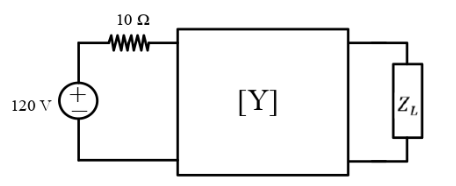
\includegraphics[width=0.5\columnwidth]{figs/Q23.png}
        \caption*{}
        \label{fig:q33}
    \end{figure}
    
    \hfill{\brak{\text{GATE EC 2023}}}
    
    \item For the circuit shown below, the propagation delay of each NAND gate is 1 ns. The critical path delay, in ns, is \underline{\hspace{2cm}} \brak{\text{rounded off to the nearest integer}}.
    \begin{figure}[H]
        \centering
        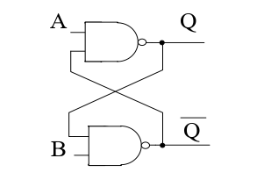
\includegraphics[width=0.6\columnwidth]{figs/Q24.png}
        \caption*{}
        \label{fig:q34}
    \end{figure}
    
    \hfill{\brak{\text{GATE EC 2023}}}
    
    \item In the circuit shown below, switch S was closed for a long time. If the switch is opened at $t=0$, the maximum magnitude of the voltage $V_R$, in volts, is \underline{\hspace{2cm}} \brak{\text{rounded off to the nearest integer}}.
    \begin{figure}[H]
        \centering
        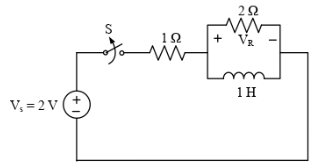
\includegraphics[width=0.4\columnwidth]{figs/Q25.png}
        \caption*{}
        \label{fig:q35}
    \end{figure}
    
    \hfill{\brak{\text{GATE EC 2023}}}
    
    \item A random variable X, distributed normally as $N\brak{0,1}$, undergoes the transformation $Y=h\brak{X}$ given in the figure. The form of the probability density function of Y is \brak{\text{In the options given below, a, b, c are non-zero constants and $g\brak{y}$ is piece-wise continuous function}}
    \begin{figure}[H]
        \centering
        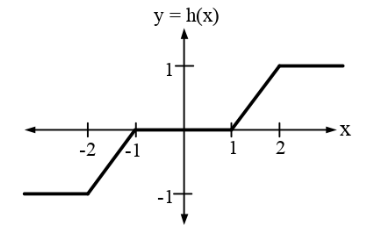
\includegraphics[width=0.4\columnwidth]{figs/Q26.png}
        \caption*{}
        \label{fig:q36}
    \end{figure}
    
    \begin{enumerate}
        \item $a\delta\brak{y-1}+b\delta\brak{y+1}+g\brak{y}$
        \item $a\delta\brak{y+1}+b\delta\brak{y}+c\delta\brak{y-1}+g\brak{y}$
        \item $a\delta\brak{y+2}+b\delta\brak{y}+c\delta\brak{y-2}+g\brak{y}$
        \item $a\delta\brak{y+2}+b\delta\brak{y-2}+g\brak{y}$
    \end{enumerate}

    \hfill{\brak{\text{GATE EC 2023}}}
    
    \item The value of the line integral $\int_{P}^{Q}\brak{z^2dx + 3y^2dy + 2xz dz}$ along the straight line joining the points $P\brak{1,1,2}$ and $Q\brak{2,3,1}$ is
    
    \begin{enumerate}
    \begin{multicols}{2}
        \item $20$
        \item $24$
        \item $29$
        \item $-5$
    \end{multicols}
    \end{enumerate}
    
    \hfill{\brak{\text{GATE EC 2023}}}
    
    \item Let x be an $n \times 1$ real column vector with length $l = \sqrt{x^T x}$. The trace of the matrix $P=xx^T$ is
    
    \begin{enumerate}
    \begin{multicols}{2}
        \item $l^2$
        \item $\frac{l^2}{4}$
        \item $l$
        \item $\frac{l^2}{2}$
    \end{multicols}
    \end{enumerate}

    \hfill{\brak{\text{GATE EC 2023}}}
    
    \item The $\frac{V_{OUT}}{V_{IN}}$ of the circuit shown below is
    \begin{figure}[H]
        \centering
        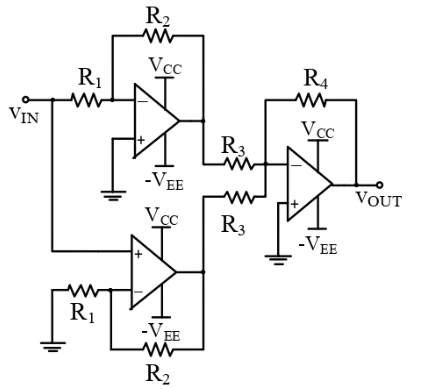
\includegraphics[width=0.7\columnwidth]{figs/Q29.png}
        \caption*{}
        \label{fig:q39}
    \end{figure}
    \begin{enumerate}
        \item $-\frac{R_4}{R_3}$
        \item $\frac{R_4}{R_3}$
        \item $1 + \frac{R_4}{R_3}$
        \item $1 - \frac{R_4}{R_3}$
    \end{enumerate}

    \hfill{\brak{\text{GATE EC 2023}}}
    
    \item In the circuit shown below, $D_1$ and $D_2$ are silicon diodes with cut-in voltage of $0.7$ V. $V_{IN}$ and $V_{OUT}$ are input and output voltages in volts. The transfer characteristic is
    \begin{figure}[H]
        \centering
        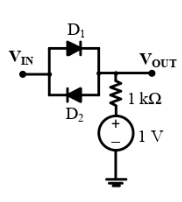
\includegraphics[width=0.4\columnwidth]{figs/Q30.png}
        \caption*{}
        \label{fig:q40}
    \end{figure}
    
    \begin{enumerate}
        \item \begin{figure}[H] \centering 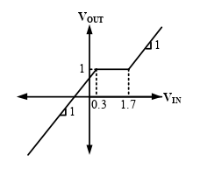
\includegraphics[width=0.4\columnwidth]{figs/Q30A.png} \caption*{} \label{fig:q40a} \end{figure}
        \item \begin{figure}[H] \centering 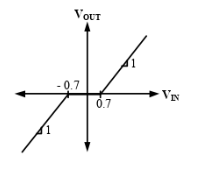
\includegraphics[width=0.4\columnwidth]{figs/Q30B.png} \caption*{} \label{fig:q40b} \end{figure}
        \item \begin{figure}[H] \centering 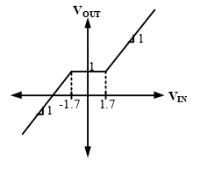
\includegraphics[width=0.4\columnwidth]{figs/Q30C.png} \caption*{} \label{fig:q40c} \end{figure}
        \item \begin{figure}[H] \centering 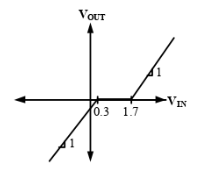
\includegraphics[width=0.4\columnwidth]{figs/Q30D.png} \caption*{} \label{fig:q40d} \end{figure}
    \end{enumerate}

    \hfill{\brak{\text{GATE EC 2023}}}
    
    \item A closed loop system is shown in the figure where $k>0$ and $\alpha>0$. The steady state error due to a ramp input $\brak{R(s)=\alpha/s^2} $is given by
    \begin{figure}[H]
        \centering
        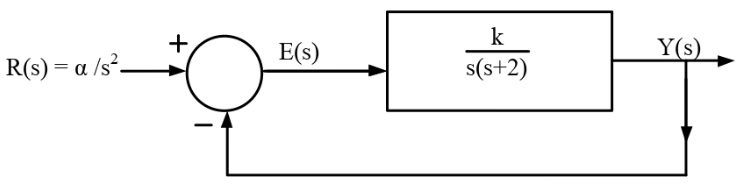
\includegraphics[width=0.6\columnwidth]{figs/Q31.png}
        \caption*{}
        \label{fig:q41}
    \end{figure}
    \begin{enumerate}
    \begin{multicols}{2}
        \item $\frac{2\alpha}{k}$
        \item $\frac{\alpha}{k}$
        \item $\frac{\alpha}{2k}$
        \item $\frac{\alpha}{4k}$
    \end{multicols}
    \end{enumerate}

    \hfill{\brak{\text{GATE EC 2023}}}
    
    \item In the following block diagram, $R(s)$ and $D(s)$ are two inputs. The output $Y(s)$ is expressed as $Y(s) = G_1(s)R(s) + G_2(s)D(s)$. $G_1(s)$ and $G_2(s)$ are given by
    \begin{figure}[H]
        \centering
        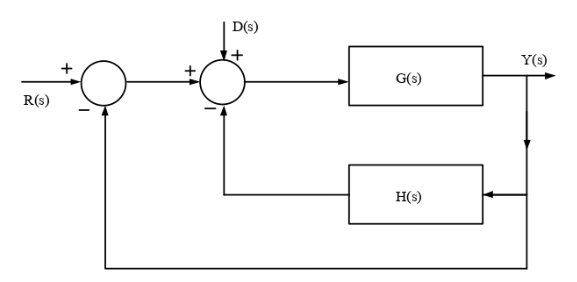
\includegraphics[width=0.6\columnwidth]{figs/Q32.png}
        \caption*{}
        \label{fig:q42}
    \end{figure}
    
    \begin{enumerate}
        \item $G_1(s) = \frac{G(s)}{1+G(s)+G(s)H(s)}$ and $G_2(s) = \frac{G(s)}{1+G(s)+G(s)H(s)}$
        \item $G_1(s) = \frac{G(s)}{1+G(s)+H(s)}$ and $G_2(s) = \frac{G(s)}{1+G(s)+H(s)}$
        \item $G_1(s) = \frac{G(s)}{1+G(s)+H(s)}$ and $G_2(s) = \frac{G(s)}{1+G(s)+G(s)H(s)}$
        \item $G_1(s) = \frac{G(s)}{1+G(s)+G(s)H(s)}$ and $G_2(s) = \frac{G(s)}{1+G(s)+H(s)}$
    \end{enumerate}

    \hfill{\brak{\text{GATE EC 2023}}}
    
    \item The state equation of a second order system is $\dot{x}(t) = Ax(t)$, $x(0)$ is the initial condition. Suppose $\lambda_1$ and $\lambda_2$ are two distinct eigenvalues of A and $v_1$ and $v_2$ are the corresponding eigenvectors. For constants $\alpha_1$ and $\alpha_2$, the solution, $x(t)$, of the state equation is

    \begin{enumerate}
        \item $\sum_{i=1}^{2}\alpha_i e^{\lambda_i t} v_i$
        \item $\sum_{i=1}^{2}\alpha_i e^{2\lambda_i t} v_i$
        \item $\sum_{i=1}^{2}\alpha_i e^{3\lambda_i t} v_i$
        \item $\sum_{i=1}^{2}\alpha_i e^{4\lambda_i t} v_i$
    \end{enumerate}

    \hfill{\brak{\text{GATE EC 2023}}}
    
    \item The switch $S_1$ was closed and $S_2$ was open for a long time. At $t=0$, switch $S_1$ is opened and $S_2$ is closed, simultaneously. The value of $i_c\brak{0^+}$, in amperes, is
    \begin{figure}[H]
        \centering
        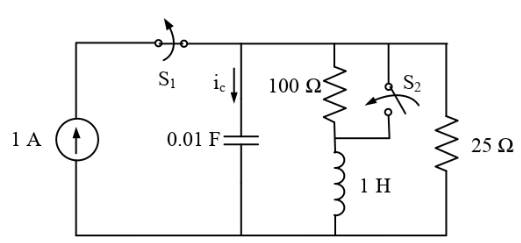
\includegraphics[width=0.5\columnwidth]{figs/Q34.png}
        \caption*{}
        \label{fig:q44}
    \end{figure}
    \begin{enumerate}
    \begin{multicols}{2}
        \item $1$
        \item $-1$
        \item $0.2$
        \item $0.8$
    \end{multicols}
    \end{enumerate}
    
    \hfill{\brak{\text{GATE EC 2023}}}
    
    \item Let a frequency modulated \brak{FM} signal $x\brak{t}=A \cos\brak{\omega_c t + k_f \int_{-\infty}^{t} m\brak{\lambda} d\lambda}$, where $m\brak{t}$ is a message signal of bandwidth W. It is passed through a non-linear system with output $y\brak{t}=2x\brak{t}+5\brak{x\brak{t}}^2$. Let $B_T$ denote the FM bandwidth. The minimum value of $\omega_c$ required to recover $x\brak{t}$ from $y\brak{t}$ is
    
    \begin{enumerate}
    \begin{multicols}{2}
        \item $B_T+W$
        \item $\frac{3}{2}B_T$
        \item $2B_T+W$
        \item $\frac{5}{2}B_T$
    \end{multicols}
    \end{enumerate}

    \hfill{\brak{\text{GATE EC 2023}}}
    
    \item The h-parameters of a two port network are shown below. The condition for the maximum small signal voltage gain $\frac{V_{out}}{V_s}$ is
    \begin{figure}[H]
        \centering
        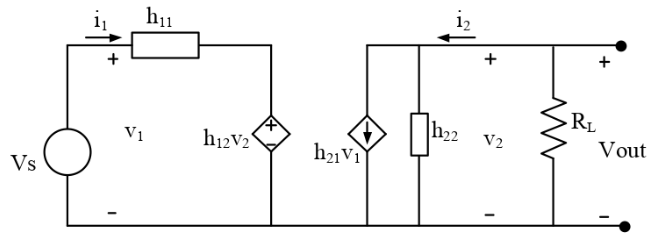
\includegraphics[width=0.7\columnwidth]{figs/Q36.png}
        \caption*{}
        \label{fig:q46}
    \end{figure}
    \begin{enumerate}
        \item $h_{11}=0, h_{12}=0, h_{21}=$ very high and $h_{22}=0$
        \item $h_{11}=$ very high, $h_{12}=0, h_{21}=$ very high and $h_{22}=0$
        \item $h_{11}=0, h_{12}=$ very high, $h_{21}=$ very high and $h_{22}=0$
        \item $h_{11}=0, h_{12}=0, h_{21}=$ very high and $h_{22}=$ very high
    \end{enumerate}

    \hfill{\brak{\text{GATE EC 2023}}}
    
    \item Consider a discrete-time periodic signal with period $N=5$. Let the discrete-time Fourier series \brak{DTFS} representation be $x[n] = \sum_{k=0}^{4} a_k e^{\frac{jk2\pi n}{5}}$, where $a_0 = 1$, $a_1=3j$, $a_2=2j$, $a_3=-2j$ and $a_4=-3j$. The value of the sum $\sum_{n=0}^{4} x[n] \sin\frac{4\pi n}{5}$ is
    \begin{enumerate}
    \begin{multicols}{2}
        \item $-10$
        \item $10$
        \item $-2$
        \item $2$
    \end{multicols}
    \end{enumerate}

    \hfill{\brak{\text{GATE EC 2023}}}
    
    \item Let an input $x[n]$ having discrete time Fourier transform $X\brak{e^{j\Omega}} = 1 - e^{-j\Omega} + 2e^{-3j\Omega}$ be passed through an LTI system. The frequency response of the LTI system is $H\brak{e^{j\Omega}} = 1 - \frac{1}{2}e^{-j2\Omega}$. The output $y[n]$ of the system is
    
    \begin{enumerate}
        \item $\delta[n]+\delta[n-1]-\frac{1}{2}\delta[n-2]-\frac{5}{2}\delta[n-3]+\delta[n-5]$
        \item $\delta[n]-\delta[n-1]-\frac{1}{2}\delta[n-2]-\frac{5}{2}\delta[n-3]+\delta[n-5]$
        \item $\delta[n]-\delta[n-1]-\frac{1}{2}\delta[n-2]+\frac{5}{2}\delta[n-3]-\delta[n-5]$
        \item $\delta[n]+\delta[n-1]+\frac{1}{2}\delta[n-2]+\frac{5}{2}\delta[n-3]+\delta[n-5]$
    \end{enumerate}

    \hfill{\brak{\text{GATE EC 2023}}}
    
    \item Let $x\brak{t} = 10 \cos\brak{10.5Wt}$ be passed through an LTI system having impulse response $h\brak{t} = \pi \brak{\frac{\sin Wt}{\pi t}}^2 \cos 10Wt$. The output of the system is
    \begin{enumerate}
    \begin{multicols}{2}
        \item $\brak{\frac{15W}{4}}\cos\brak{10.5Wt}$
        \item $\brak{\frac{15W}{2}}\cos\brak{10.5Wt}$
        \item $\brak{\frac{15W}{8}}\cos\brak{10.5Wt}$
        \item $\brak{15W}\cos\brak{10.5Wt}$
    \end{multicols}
    \end{enumerate}
    
    \hfill{\brak{\text{GATE EC 2023}}}
    
    \item Let $x_1(t)$ and $x_2(t)$ be two band-limited signals having bandwidth $B = 4\pi \times 10^3$ rad/s each. In the figure below, the Nyquist sampling frequency, in rad/s, required to sample $y(t)$, is
    \begin{figure}[H]
        \centering
        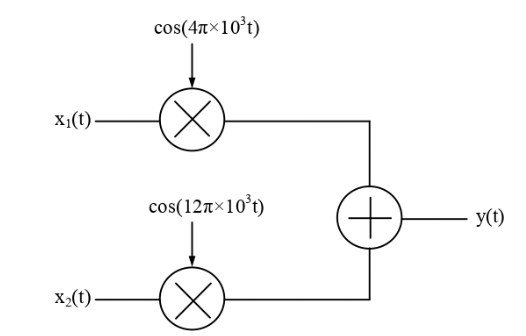
\includegraphics[width=0.7\columnwidth]{figs/Q40.png}
        \caption*{}
        \label{fig:q50}
    \end{figure}
    \begin{enumerate}
        \begin{multicols}{2}
            \item $20\pi \times 10^3$
            \item $40\pi \times 10^3$
            \item $8\pi \times 10^3$
            \item $32\pi \times 10^3$
        \end{multicols}
    \end{enumerate}
    
    \hfill{\brak{\text{GATE EC 2023}}}
    
    \item The S-parameters of a two port network is given as
    \[ [S] = \myvec{S_{11} & S_{12} \\ S_{21} & S_{22}} \]
    with reference to $Z_0$. Two lossless transmission line sections of electrical lengths $\theta_1 = \beta l_1$ and $\theta_2 = \beta l_2$ are added to the input and output ports for measurement purposes, respectively. The S-parameters $[S']$ of the resultant two port network is
    \begin{figure}[H]
        \centering
        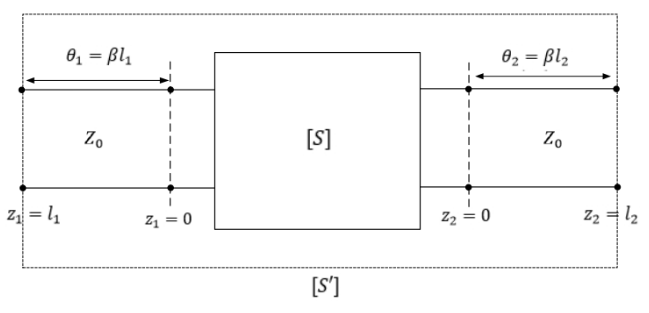
\includegraphics[width=0.8\columnwidth]{figs/Q41.png}
        \caption*{}
        \label{fig:q51}
    \end{figure}
    
    \begin{enumerate}
        \item $\myvec{S_{11}e^{-j2\theta_1} & S_{12}e^{-j(\theta_1+\theta_2)} \\ S_{21}e^{-j(\theta_1+\theta_2)} & S_{22}e^{-j2\theta_2}}$
        \item $\myvec{S_{11}e^{j2\theta_1} & S_{12}e^{-j(\theta_1+\theta_2)} \\ S_{21}e^{-j(\theta_1+\theta_2)} & S_{22}e^{j2\theta_2}}$
        \item $\myvec{S_{11}e^{j2\theta_1} & S_{12}e^{j(\theta_1+\theta_2)} \\ S_{21}e^{j(\theta_1+\theta_2)} & S_{22}e^{j2\theta_2}}$
        \item $\myvec{S_{11}e^{-j2\theta_1} & S_{12}e^{j(\theta_1+\theta_2)} \\ S_{21}e^{j(\theta_1+\theta_2)} & S_{22}e^{-j2\theta_2}}$
    \end{enumerate}
    
    \hfill{\brak{\text{GATE EC 2023}}}

    \item The standing wave ratio on a 50 $\Omega$ lossless transmission line terminated in an unknown load impedance is found to be 2.0. The distance between successive voltage minima is 30 cm and the first minimum is located at 10 cm from the load. $Z_L$ can be replaced by an equivalent length $l_m$ and terminating resistance $R_m$ of the same line. The value of $R_m$ and $l_m$, respectively, are
    \begin{figure}[H]
        \centering
        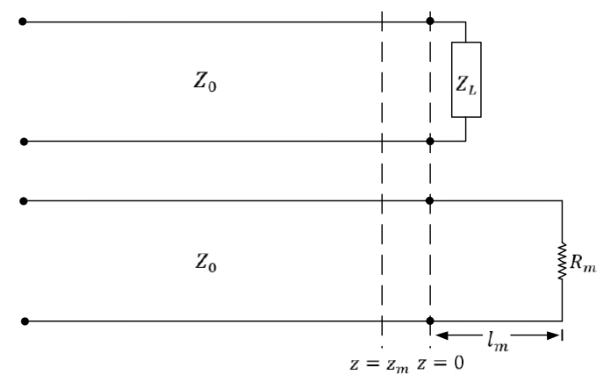
\includegraphics[width=0.7\columnwidth]{figs/Q42.png}
        \caption*{}
        \label{fig:q52}
    \end{figure}
    
    \begin{enumerate}
        \item $R_m = 100 \Omega$, $l_m = 20$ cm
        \item $R_m = 25 \Omega$, $l_m = 20$ cm
        \item $R_m = 100 \Omega$, $l_m = 5$ cm
        \item $R_m = 25 \Omega$, $l_m = 5$ cm
    \end{enumerate}
    
    \hfill{\brak{\text{GATE EC 2023}}}
    
    \item The electric field of a plane electromagnetic wave is
    $E = a_x C_{1x} \cos(\omega t - \beta z) + a_y C_{1y} \cos(\omega t - \beta z + \theta) V/m$.
    Which of the following combination(s) will give rise to a left handed elliptically polarized (LHEP) wave?
    
    \begin{enumerate}
        \item $C_{1x}=1, C_{1y}=1, \theta=\pi/4$
        \item $C_{1x}=2, C_{1y}=1, \theta=\pi/2$
        \item $C_{1x}=1, C_{1y}=2, \theta=3\pi/2$
        \item $C_{1x}=2, C_{1y}=1, \theta=3\pi/4$
    \end{enumerate}

    \hfill{\brak{\text{GATE EC 2023}}}
    
    \item The following circuit(s) representing a lumped element equivalent of an infinitesimal section of a transmission line is/are
    
    \begin{enumerate}
        \item \begin{figure}[H] \centering 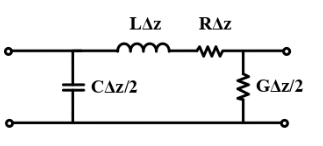
\includegraphics[width=0.4\columnwidth]{figs/Q44A.png} \caption*{} \label{fig:q40a} \end{figure}
        \item \begin{figure}[H] \centering 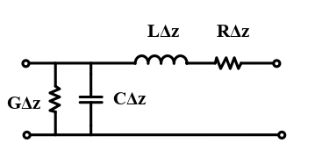
\includegraphics[width=0.4\columnwidth]{figs/Q44B.png} \caption*{} \label{fig:q40b} \end{figure}
        \item \begin{figure}[H] \centering 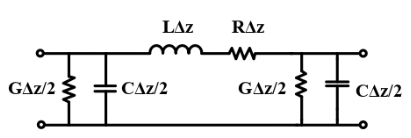
\includegraphics[width=0.4\columnwidth]{figs/Q44C.png} \caption*{} \label{fig:q40c} \end{figure}
        \item \begin{figure}[H] \centering 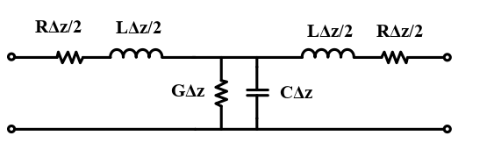
\includegraphics[width=0.4\columnwidth]{figs/Q44D.png} \caption*{} \label{fig:q40d} \end{figure}
    \end{enumerate}
    
    \hfill{\brak{\text{GATE EC 2023}}}
    
    \item The value of the integral $\iint_R xy \, dx \, dy$ over the region R, given in the figure, is \underline{\hspace{2cm}} \\\brak{\text{rounded off to the nearest integer}.}
    \begin{figure}[H]
        \centering
        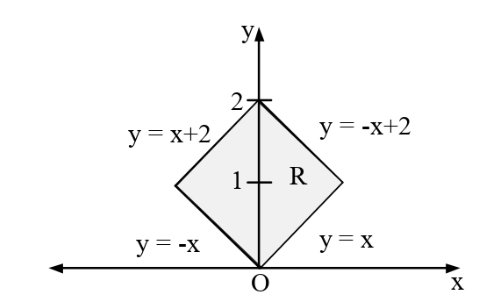
\includegraphics[width=0.4\columnwidth]{figs/Q45.png}
        \caption*{}
        \label{fig:q55}
    \end{figure}
    
    \hfill{\brak{\text{GATE EC 2023}}}
    
    \item In an extrinsic semiconductor, the hole concentration is given to be $1.5n_i$ where $n_i$ is the intrinsic carrier concentration of $1 \times 10^{10} cm^{-3}$. The ratio of electron to hole mobility for equal hole and electron drift current is given as \underline{\hspace{2cm}} \brak{\text{rounded off to two decimal places}.}
    
    \hfill{\brak{\text{GATE EC 2023}}}
    
    \item The asymptotic magnitude Bode plot of a minimum phase system is shown in the figure. The transfer function of the system is $G(s) = \frac{k(s+z)^a}{s^b(s+p)^c}$, where k, z, p, a, b and c are positive constants. The value of $(a+b+c)$ is \underline{\hspace{2cm}} \brak{\text{rounded off to the nearest integer}.}
    \begin{figure}[H]
        \centering
        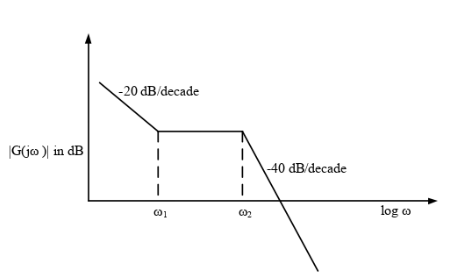
\includegraphics[width=0.6\columnwidth]{figs/Q47.png}
        \caption*{}
        \label{fig:q57}
    \end{figure}
    
    \hfill{\brak{\text{GATE EC 2023}}}
    
    \item Let $x_1(t) = u(t+1.5) - u(t-1.5)$ and $x_2(t)$ is shown in the figure below. For $y(t) = x_1(t) * x_2(t)$, the $\int_{-\infty}^{\infty} y(t) dt$ is \underline{\hspace{2cm}} \brak{\text{rounded off to the nearest integer}.}
    \begin{figure}[H]
        \centering
        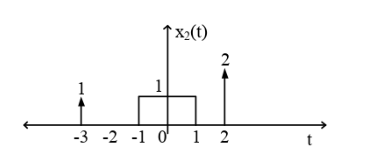
\includegraphics[width=0.4\columnwidth]{figs/Q48.png}
        \caption*{}
        \label{fig:q58}
    \end{figure}
    
    \hfill{\brak{\text{GATE EC 2023}}}
    
    \item Let $X(t)$ be a white Gaussian noise with power spectral density $\frac{1}{2}$ W/Hz. If $X(t)$ is input to an LTI system with impulse response $e^{-t}u(t)$. The average power of the system output is \underline{\hspace{2cm}} W\\ \brak{\text{rounded off to two decimal places}}.
    
    \hfill{\brak{\text{GATE EC 2023}}}
    
    \item A transparent dielectric coating is applied to glass $\brak{\epsilon_r = 4, \mu_r = 1} $to eliminate the reflection of red light $\brak{\lambda_0 = 0.75 \mu m}$. The minimum thickness of the dielectric coating, in $\mu$m, that can be used is \underline{\hspace{2cm}} \brak{\text{rounded off to two decimal places}.}
    
    \hfill{\brak{\text{GATE EC 2023}}}
    
    \item In a semiconductor device, the Fermi-energy level is $0.35$ eV above the valence band energy. The effective density of states in the valence band at $T=300$ K is $1 \times 10^{19} cm^{-3}$. The thermal equilibrium hole concentration in silicon at 400 K is \underline{\hspace{2cm}} $\times 10^{13} cm^{-3}$ \brak{\text{rounded off to two decimal places}.}
    
    Given kT at 300 K is 0.026 eV.
    
    \hfill{\brak{\text{GATE EC 2023}}}
    
    \item A sample and hold circuit is implemented using a resistive switch and a capacitor with a time constant of 1 $\mu$s. The time for the sampling switch to stay closed to charge a capacitor adequately to a full scale voltage of 1 V with 12-bit accuracy is \underline{\hspace{2cm}} $\mu$s \brak{\text{rounded off to two decimal places}.}
    
    \hfill{\brak{\text{GATE EC 2023}}}
    
    \item In a given sequential circuit, initial states are $Q_1=1$ and $Q_2=0$. For a clock frequency of 1 MHz, the frequency of signal $Q_2$ in kHz, is \underline{\hspace{2cm}} \brak{\text{rounded off to the nearest integer}}.
    \begin{figure}[H]
        \centering
        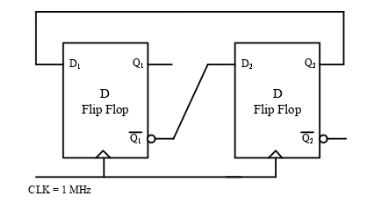
\includegraphics[width=0.5\columnwidth]{figs/Q53.png}
        \caption*{}
        \label{fig:q63}
    \end{figure}
    
    \hfill{\brak{\text{GATE EC 2023}}}
    
    \item In the circuit below, the voltage $V_L$ is \underline{\hspace{2cm}} V \brak{\text{rounded off to two decimal places}}.
    \begin{figure}[H]
        \centering
        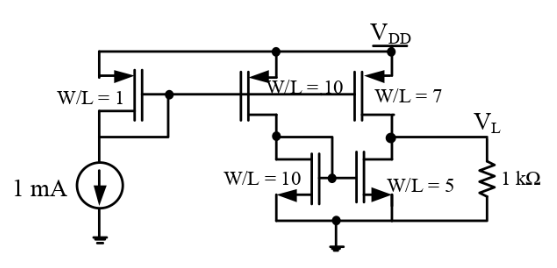
\includegraphics[width=0.6\columnwidth]{figs/Q54.png}
        \caption*{}
        \label{fig:q64}
    \end{figure}
    
    \hfill{\brak{\text{GATE EC 2023}}}
    
    \item The frequency of occurrence of 8 symbols (a-h) is shown in the table below. A symbol is chosen and it is determined by asking a series of "yes/no" questions which are assumed to be truthfully answered. The average number of questions when asked in the most efficient sequence, to determine the chosen symbol, is \underline{\hspace{2cm}} \brak{\text{rounded off to two decimal places}.}
    \begin{table}[H]
        \centering
        \begin{tabular}{|c|c|c|c|c|c|c|c|c|}
            \hline
            \textbf{Symbols} & a & b & c & d & e & f & g & h \\
            \hline
            \textbf{Frequency of occurrence} & $\frac{1}{2}$ & $\frac{1}{4}$ & $\frac{1}{8}$ & $\frac{1}{16}$ & $\frac{1}{32}$ & $\frac{1}{64}$ & $\frac{1}{128}$ & $\frac{1}{128}$ \\
            \hline
        \end{tabular}
    \end{table}
    \hfill{\brak{\text{GATE EC 2023}}}

\end{enumerate}

\end{document}

